% Created 2023-10-09 Mon 15:38
% Intended LaTeX compiler: pdflatex
\documentclass[11pt]{article}
\usepackage[utf8]{inputenc}
\usepackage[T1]{fontenc}
\usepackage{graphicx}
\usepackage{longtable}
\usepackage{wrapfig}
\usepackage{rotating}
\usepackage[normalem]{ulem}
\usepackage{amsmath}
\usepackage{amssymb}
\usepackage{capt-of}
\usepackage{hyperref}
\usepackage{alltt}
\usepackage[utf8]{inputenc}
\usepackage{mdwlist}
\usepackage{amssymb}
\usepackage[fleqn]{mathtools}
\usepackage{multicol}
\usepackage{enumitem}
\usepackage[dvipsnames]{xcolor}
\usepackage{wrapfig}
\usepackage{array}
\usepackage{nccmath}
\usepackage{graphicx}
\usepackage{fancyhdr}
\usepackage{tikz}
\usepackage[margin=0.5in]{geometry}
\usepackage{fdsymbol}
\pgfdeclarelayer{background}
\pgfdeclarelayer{foreground}
\pgfsetlayers{background,main,foreground}
\newcommand{\done}{$\quad\blacksquare$}
\newcommand{\lSeq}[1]{\left\{#1_n\right\}^{\infty}_{n=1}}
\newcommand{\lHed}[1]{\noindent\textbf{#1}}
\newcommand{\0}{\emptyset}
\newcommand{\N}{\mathbb{N}}
\newcommand{\Z}{\mathbb{Z}}
\newcommand{\Q}{\mathbb{Q}}
\newcommand{\R}{\mathbb{R}}
\newcommand{\C}{\mathbb{C}}
\newcommand{\lcm}{\text{lcm}}
\newcommand{\Unif}{\text{Unif}}
\newcommand{\Ber}{\text{Ber}}
\newcommand{\Binom}{\text{Binom}}
\newcommand{\Pois}{\text{Pois}}
\DeclareMathOperator{\proj}{proj}
\DeclareMathOperator{\vspan}{span}
\DeclareMathOperator{\Log}{Log}
\DeclareMathOperator*{\Res}{Res}
\date{}
\title{Algebra I}
\hypersetup{
 pdfauthor={},
 pdftitle={Algebra I},
 pdfkeywords={},
 pdfsubject={},
 pdfcreator={Emacs 29.1 (Org mode 9.7)}, 
 pdflang={English}}
\begin{document}

\maketitle
\section*{September 28, 2023}
\label{sec:org34070e0}
\subsection*{Grade Weights}
\label{sec:orgde0ddfc}
50\% Homework + 50\% Final\\[0pt]
Participation matters for pass/fail.\\[0pt]
\subsection*{Office Hours}
\label{sec:orgb58394d}
Tuesday / Thursday 11:25 - 12:00\\[0pt]
Or by appointment (jusuh@ucsc.edu)\\[0pt]
\subsection*{Recommended Text}
\label{sec:orgcb5d7be}
Abstract Algebra (3e) - Dummit and Foote\\[0pt]
Finite Groups: An Introduction (2nd revised) - Jean-Pierre Serre\\[0pt]
Robert Boltje's Lecture Notes - (\url{https://boltje.math.ucsc.edu/courses/f17/f17m200notes.pdf})\\[0pt]
\subsection*{Binary Operation}
\label{sec:org4b44257}
Let \(S\) be a set. A binary operation on \(S\) is a function \(f:S\times S\to S\). We will almost never use \(f\) for the binary operation (\(f(s,t)\)).\\[0pt]
The usual notation for binary operations is \(s*t\).\\[0pt]
\subsubsection*{Example}
\label{sec:org4c51b51}
\begin{enumerate}
\item \(S=\R^{3}\), define \(f:S\times S\to S\) as \((\vec{x}, \vec{y}) \rightsquigarrow \vec{x}+\vec{y}\).\\[0pt]
\item \(S=\R^{3}\), define \(S\times S\overset{f}{\to} S\) as \((\vec{x},\vec{y})\rightsquigarrow\vec{x}+\vec{y}\).\\[0pt]
\begin{itemize}
\item Note that \((\vec{x},\vec{y})\rightsquigarrow\vec{x}\cdot\vec{y}\) is not a binary operation.\\[0pt]
\end{itemize}
\item \(S=\Z\) as \((m,n)\mapsto m\cdot n\).\\[0pt]
\item \(S=\R^{3}\) as \((\vec{x},\vec{y})\rightsquigarrow\frac{\vec{x}+\vec{y}}{2}\)\\[0pt]
\begin{tikzpicture}
  \node (0) at (0,0) {};
  \node (x) at (0,1) {};
  \node (y) at (1,0) {};
  \node (xy) at ({1/2},{1/2}) {};
  \draw[->] (0.center) to (x.center);
  \draw[->] (0.center) to (y.center);
  \draw[->] (0.center) to (xy.center);
\end{tikzpicture}
\item Let \(n\geq 1\) be an interger and \(S= M_{n\times n}(\R)=\{n\times n\text{ real matricies}\}\). Then \((A,B)\rightsquigarrow AB\).\\[0pt]
\end{enumerate}
\subsubsection*{Observations}
\label{sec:orgc756032}
Examples 1,3,5 are associative; examples 2,4 are not.\\[0pt]
Examples 1-4 are commutative; example 5 commutes only when \(n=1\).\\[0pt]
\(\vec{0}\) for example 1, \(1\) for example 3, and \(I_{n}\) for example 5.\\[0pt]
\subsection*{Q: What is a Group?}
\label{sec:orgf41cf08}
A \href{../Definitions/group.org}{group} is a set equipped with a binary operation which satisfies three axioms.\\[0pt]
Let \(*\) be a binary operation on a set \(S\).\\[0pt]
\begin{enumerate}
\item Say \(*\) is associative if \(\forall a,b,c\in S\), \((a*b)*c=a*(b*c)\).\\[0pt]
\item Say \(*\) is commutative if \(\forall a,b\in S\), \(a*b=b*a\).\\[0pt]
\item An element \(e\in S\) is a neutral element (with respect to \(*\)) if \(\forall a\in S\), \(a*e=a=e*a\).\\[0pt]
\begin{itemize}
\item If there exists a neutral element, then it is unique.\\[0pt]
\end{itemize}
\item Suppose \((S,*)\) has a neutral element \(e\). Let \(a\in S\). Then \(b\in S\) is called an inverse of \(a\) (with respect to \(*\)) if \(a*b=e=b*a\).\\[0pt]
\end{enumerate}
\subsection*{Group}
\label{sec:org3072b24}
A group is a set \(G\) equipped with a binary operation \(*\) such that\\[0pt]
\begin{enumerate}
\item \(*\) is associative.\\[0pt]
\item \(*\) has a neutral element \(e\).\\[0pt]
\item Every \(g\in G\) has an inverse.\\[0pt]
\end{enumerate}
If, in addition, \(*\) is commutative, we say \((G,*)\) is an abelian or commutative group.\\[0pt]
\subsubsection*{Examples}
\label{sec:orgd160984}
\((\R^{3},+)\) is a commutative group.\\[0pt]
\((\R^{3},\times)\) has no neutral element.\\[0pt]
\((\Z,\cdot)\) has no inverse (except \(\pm 1\)).\\[0pt]
\((\R^{3},\text{mid})\) is not associative. (the midpoint)\\[0pt]
\((M_{n\times n}(\R),\cdot)\) has no inverse of \(0_{n\times n}\).\\[0pt]
For \(n\geq 1\), \((\R^{n},+)\) and \((\C^{n},+)\) are abelian groups.\\[0pt]
\subsubsection*{Proof that the Neutral Element is unique.}
\label{sec:org91f6295}
Let \(e,e'\) be neutral eements. Then \(e'=e*e'=e\). \(\blacksquare\)\\[0pt]
\subsubsection*{Proof that the Inverse is unique.}
\label{sec:org872ae1e}
Left to the reader.\\[0pt]
\subsection*{Subgroup}
\label{sec:org2be8482}
Let \(G\) be a group, and let \(H\) be a subset of \(G\). We say that \(H\) is a subgroup of \(G\) if\\[0pt]
\begin{enumerate}
\item \(\forall h_{1},h_{2}\in H\), \(h_{1}*h_{2}\in H\).\\[0pt]
\item \(e\in H\).\\[0pt]
\item \(\forall h\in H\), \(h^{-1}\in H\).\\[0pt]
\end{enumerate}
\subsubsection*{Examples}
\label{sec:org2c4d9a6}
\(\Z^{n}\subseteq \R^{n}\) is a subgroup \((*=+)\).\\[0pt]
\(G=\{A\in M_{n\times n}:\det(A)\neq 0\}\). Then \((G,\cdot)\) is a group.\\[0pt]
\begin{itemize}
\item This is the General Linear Group on \(\R\): \(\text{GL}_{n}(\R)\).\\[0pt]
\item Recall \(A^{-1}=\frac{1}{\det(A)}\left( (-1)^{itj}\det(M_{\alpha_{i}}) \right)\).\\[0pt]
\end{itemize}
\subsection*{General Linear Subgroups}
\label{sec:org2dc6011}
\(S=\{A\in\text{GL}_{n}(\R):a_{ij}\in\Z,\;\forall 1\leq i,j\leq n\}\).\\[0pt]
\(S\) is closed under \(\cdot\) and \(I_{n}\in S\), but for example\\[0pt]
\begin{align*}
  \begin{pmatrix}
    1 & 2 \\
    3 & 4
  \end{pmatrix}^{-1}
  = \frac{1}{1\cdot4-2\cdot3}
  \begin{pmatrix}
    4 & -2 \\
    -3 & 1
  \end{pmatrix}
  =
  \begin{pmatrix}
    -2 & 1 \\
    \frac{3}{2} & -\frac{1}{2}
  \end{pmatrix}
\end{align*}
so \(S\) is not a subgroup.\\[0pt]
However, \(T=\{A\in S:\det(A)=\pm1\} \subseteq \text{GL}_{n}(\R)\).\\[0pt]
\begin{itemize}
\item Note that if \(AA'=I_{n}\) then \(\det(A)\det(A')=1\).\\[0pt]
\end{itemize}
\subsection*{Additive Groups}
\label{sec:orgc66d898}
For groups like \(\Z^{n}\), \(\R^{n}\) and \(\C^{n}\), we will use \(+\) for the binary operation and say that they are additive groups.\\[0pt]
The Neutral Element is denoted as \(0\).\\[0pt]
The inverse is denoted as \(-g\).\\[0pt]
For \(m\geq 1\) and \(g\in G\), \(mg=g+\overset{m}{\cdots}+g\) and \((-m)g=-(mg)\).\\[0pt]
\subsection*{Multiplicative Groups}
\label{sec:org64b5899}
For groups like \(\text{GL}_{n}(\C)\) or \(\text{GL}_{n}(\Z)\), we say that the group is multiplicative.\\[0pt]
Denote the neutral element as \(1\).\\[0pt]
Denote the inverse of \(g\) as \(g^{-1}\).\\[0pt]
For \(m\geq1\), \(g^{m}=g\overset{m}{\cdots}g\).\\[0pt]
\(g^{0}=1\).\\[0pt]
\(g^{-m}=(g^{m})^{-1}\).\\[0pt]
\subsection*{Group Element Order}
\label{sec:org0f3f59d}
Let \(G\) be a group, \(g\in G\), and \(m\geq 1\).\\[0pt]
Say \(g\) has order \(m\) if \(g^{m}=1\) and \(g^{k}\neq 1,\;\forall k\) such that \(1\leq k\leq m\).\\[0pt]
An element has infinite order if \(g^{m}\neq1,\;\forall m\in\Z^{+}\).\\[0pt]
\subsubsection*{Examples}
\label{sec:org903f514}
In \(D_{10}\), \(I_{2}\) has order \(1\), rotations have order \(5\) and reflections have order \(2\).\\[0pt]
\subsection*{Groups from Geometry}
\label{sec:org3b9cce8}
\subsubsection*{Pentagon}
\label{sec:orgcd6486b}
Consider the regular pentagon \(P\).\\[0pt]

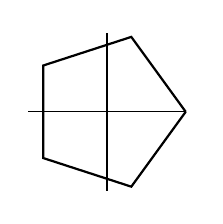
\begin{tikzpicture}
  \node (A) at (1,0) {};
  \node (B) at ({cos(72)},{sin(72)}) {};
  \node (C) at ({cos(144)},{sin(144)}) {};
  \node (D) at ({cos(216)},{sin(216)}) {};
  \node (E) at ({cos(288)},{sin(288)}) {};
  \draw (-1,0) -- (1,0);
  \draw (0,-1) -- (0,1);
  \draw[thick] (A.center) -- (B.center) -- (C.center) -- (D.center) -- (E.center) -- (A.center);
\end{tikzpicture}

\(H=\{T\in\text{GL}_{2}(\R):T(P)=P\}\).\\[0pt]
This is the symmetry group of \(P\) or \(D_{10}\) (sometimes \(D_{5}\))\\[0pt]
\(H\leq\text{GL}_{2}(\R)\).\\[0pt]
\begin{itemize}
\item Proof of closure.
\label{sec:orga1a44ab}
Suppose \(T_{1},T_{2}\in H\). Then \(T_{1}(P)=P\), \(T_{2}(P)=P\) and \((T_{1}\circ T_{2})(P)=T_{1}(T_{2}(P))=T_{1}(P)=P\).\\[0pt]
Therefore \(H\) is closed under \(\circ\).\\[0pt]
\item Proof of identity.
\label{sec:orgaa38239}
\(\text{Id}_{\text{GL}_{2}}=I_{2}\) does satisfy \(I_{2}(P)\).\\[0pt]
\item Proof of inverse.
\label{sec:orgf1e1540}
If \(T\in H\) (i.e. \(T\in\text{GL}_{2}(\R)\) and \(T(P)=P\), apply \(T^{-1}\) and get \(T^{-1}(T(P))=T^{-1}(P)\). Therefore \(P=T^{-1}(P)\).\\[0pt]
\end{itemize}
\subsubsection*{Tetrahedron}
\label{sec:orgc14f5b7}
Let \(X\) be the regular tetrahedron and \(A=\{\text{rotational symmetries of } X\}\).\\[0pt]
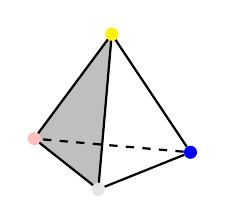
\begin{tikzpicture}
  \begin{scope}[nodes = {fill, circle, scale = 0.5}, font = \LARGE]
    \node[blue] (a) at ({cos(0)},{sin(0)}) {};
    \node[pink] (b) at ({cos(170)},{sin(170)}) {};
    \node[gray!20] (c) at ({0.5*cos(250)},{0.5*sin(250)}) {};
    \node[yellow] (d) at ({1.5*cos(90)},{1.5*sin(90)}) {};
  \end{scope}
  \begin{pgfonlayer}{background}
  \path [fill=lightgray,draw] (b.center) to (c.center) to (d.center) to (b.center);
  \end{pgfonlayer}
  \begin{scope}[thick]
    \draw (a) -- (c) -- (b) -- (d) -- (a);
    \draw [dashed] (a) -- (b);
    \draw (c) -- (d);
  \end{scope}
\end{tikzpicture}
Then \(A\) contains\\[0pt]
\begin{itemize}
\item The identity: 1.\\[0pt]
\item \(2\cdot 4=8\) rotations by \(120^{\circ}\).\\[0pt]
\item 3 rotations of \(180^{\circ}\).\\[0pt]
\end{itemize}
So we have a bijection \(r:\{B,P,W,Y\}\to\{B,P,W,Y\}\) where\\[0pt]
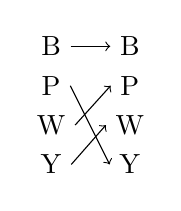
\begin{tikzpicture}
  \node (bl) at ({-1/2},2) {B};
  \node (pl) at ({-1/2},{3/2}) {P};
  \node (wl) at ({-1/2},1) {W};
  \node (yl) at ({-1/2},{1/2}) {Y};
  \node (br) at ({1/2},2) {B};
  \node (pr) at ({1/2},{3/2}) {P};
  \node (wr) at ({1/2},1) {W};
  \node (yr) at ({1/2},{1/2}) {Y};
  \draw[->] (bl.east) to (br.west);
  \draw[->] (pl.east) to (yr.west);
  \draw[->] (wl.east) to (pr.west);
  \draw[->] (yl.east) to (wr.west);
\end{tikzpicture}
\subsection*{Symmetric Group}
\label{sec:org99921ef}
Let \(S\) be a set (e.g. \(E=\{B,P,W,Y\}\)). The Symmetric Group \(\text{Sym}(E)\) is the set of bijections \(f:E\to E\) equipped with the binary operation \(\circ\) (composition).\\[0pt]
\section*{October 3, 2023}
\label{sec:orgeca060c}
\subsection*{Homework}
\label{sec:orgdff9a4f}
First homework should be released this Thursday, October 5th.\\[0pt]
Next lecture will be on group actions.\\[0pt]
\subsection*{Symmetric Group}
\label{sec:org590bebe}
Let \(X\) be a set.\\[0pt]
When \(|X|=n\) denote the elements \(\{1,2,\ldots,n\}\).\\[0pt]
\(\text{Sym}(X)=\{f:X\to X|f\text{ is bijective}\}\).\\[0pt]
With \(\circ\) (composition of functions) as a binary operation, \(\text{Sym}(X)\) is a group.\\[0pt]
\subsubsection*{Symmetric Group Order}
\label{sec:org7562119}
If \(|X|=n\), then \(|\text{Sym}(X)|=n!\)\\[0pt]
\begin{itemize}
\item Proof
\label{sec:orgbf94cc4}
Let \(X=\{1,2,\ldots,n\}\). A bijection \(f\) consists of \(f(1),f(2),\ldots,f(n)\).\\[0pt]
For \(f(1)\), we have \(n\) choices; for \(f(2)\) we have \(n-1\) choices. This continues until only \(1\) choice remains for \(f(n)\).\\[0pt]
Therefore the choices are \((n)(n-1)\cdots(1)=n!\)\\[0pt]
\end{itemize}
\subsubsection*{Example}
\label{sec:orgce656e0}
For the symmetric group on four letters \(\{a,b,c,d\}\), \(|\text{Sym}(4)|=4!=24\)\\[0pt]
\subsection*{Cycles}
\label{sec:org198e332}
Let \(x=\{1,\ldots,n\}\), \(m\geq1\) be an integer and \(a_{1},a_{2},\ldots,a_{m}\) distinct elements in \(X\).\\[0pt]
Then the m-cycle denoted by \((a_{1}\;a_{2}\;\cdots\;a_{m})\) is the element of \(\text{Sym}(X)\) which maps \(a_{1}\) to \(a_{2}\), \(a_{2}\) to \(a_{3}\),\ldots{}, \(a_{m-1}\) to \(a_{m}\), and \(a_{m}\) to \(a_{1}\).\\[0pt]
\subsubsection*{Example}
\label{sec:org27bbc93}
Let \(n=7\) and \(m=4\). Then \((2\;7\;1\;3)\) is a bijection.\\[0pt]
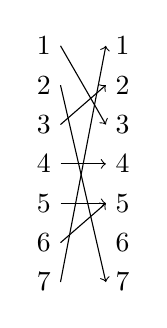
\begin{tikzpicture}
  \node (1l) at ({-1/2},2) {1};
  \node (2l) at ({-1/2},{3/2}) {2};
  \node (3l) at ({-1/2},1) {3};
  \node (4l) at ({-1/2},{1/2}) {4};
  \node (5l) at ({-1/2},0) {5};
  \node (6l) at ({-1/2},{-1/2}) {6};
  \node (7l) at ({-1/2},-1) {7};
  \node (1r) at ({1/2},2) {1};
  \node (2r) at ({1/2},{3/2}) {2};
  \node (3r) at ({1/2},1) {3};
  \node (4r) at ({1/2},{1/2}) {4};
  \node (5r) at ({1/2},0) {5};
  \node (6r) at ({1/2},{-1/2}) {6};
  \node (7r) at ({1/2},-1) {7};
  \draw[->] (1l.east) to (3r.west);
  \draw[->] (2l.east) to (7r.west);
  \draw[->] (3l.east) to (2r.west);
  \draw[->] (4l.east) to (4r.west);
  \draw[->] (5l.east) to (5r.west);
  \draw[->] (6l.east) to (5r.west);
  \draw[->] (7l.east) to (1r.west);
\end{tikzpicture}
\subsubsection*{Degenerate Case}
\label{sec:org4e06d9d}
\(m=1\) gives \(\text{Id}_{X}\).\\[0pt]
\subsubsection*{First Non-Degenerate Case}
\label{sec:orgb5efa0d}
A transposition is, by definition a 2-cycle: \((a_{1}\;a_{2})\).\\[0pt]
\subsubsection*{Symmetric Group as Cycle Composition}
\label{sec:org6b9b847}
Every elenent in \(\text{Sym}(X)\) is the product (using \(\circ\)) of m-cycles, where m can vary.\\[0pt]
\begin{itemize}
\item Proof
\label{sec:org25609ae}
Consider \(\text{Sym}(6)\).\\[0pt]
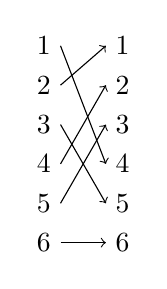
\begin{tikzpicture}
  \node (1l) at ({-1/2},2) {1};
  \node (2l) at ({-1/2},{3/2}) {2};
  \node (3l) at ({-1/2},1) {3};
  \node (4l) at ({-1/2},{1/2}) {4};
  \node (5l) at ({-1/2},0) {5};
  \node (6l) at ({-1/2},{-1/2}) {6};
  \node (1r) at ({1/2},2) {1};
  \node (2r) at ({1/2},{3/2}) {2};
  \node (3r) at ({1/2},1) {3};
  \node (4r) at ({1/2},{1/2}) {4};
  \node (5r) at ({1/2},0) {5};
  \node (6r) at ({1/2},{-1/2}) {6};
  \draw[->] (1l.east) to (4r.west);
  \draw[->] (2l.east) to (1r.west);
  \draw[->] (3l.east) to (5r.west);
  \draw[->] (4l.east) to (2r.west);
  \draw[->] (5l.east) to (3r.west);
  \draw[->] (6l.east) to (6r.west);
\end{tikzpicture}
This gives a bijection \(\pi = (1\;4\;2)(3\;5)(6)\) which is the composition of cycles.\\[0pt]
We say that this \(\pi\) has cycle type \(3+2+1\).\\[0pt]
\item Cycle Type
\label{sec:orgd4b43b9}
If instead \(\pi=(1\;4\;2)(3\;5\;6)\) then the cycle type is given as \(3+3\).\\[0pt]
\end{itemize}
\subsection*{Finite Symmetric Groups}
\label{sec:orge7ee866}
For \(n=2\), \(\text{Sym}(X)=\{\text{Id},(1\;2)\}\).\\[0pt]
This gives cylce types \(1+1\) and \(2\).\\[0pt]
For \(n=3\), \(\text{Sym}(X)=\{\text{Id},(1\;2),(1\;3),(2\;3),(1\;2\;3),(1\;3\;2)\}\).\\[0pt]
This gives cycle types \(1+1\), \(2+1\) and \(3\).\\[0pt]
\subsection*{Symmetric Group for Tetrahedron}
\label{sec:org28796b9}
For \(n=4\) let \(X=\{B,P,W,Y\}\).\\[0pt]
Partitions of \(n=4\) are\\[0pt]
\begin{align*}
  4
  &=4 && 6 && (B\;P\;W\;Y) && \cdots && && && && && \text{sign}=-1
  \\&=3+1 && 4\cdot 2=8 && (P\;W\;Y) && \cdots && && && && && \text{sign}=+1
  \\&=2+2 && \frac{\binom{4}{2}}{2}=3 && (B\;P)(W\;Y) && (B\;W)(P\;Y) && (B\;Y)(P\;W) && && && && \text{sign}=+1
  \\&=2+1+1 && \binom{4}{2}=6 && (B\;P) && (B\;W) && (B\;Y) && (P\;W) && (P\;Y) && (W\;Y) && \text{sign}=-1
  \\&=1+1+1+1 && 1 && \text{Id}_{X} && && && && && && \text{sign}=+1
\end{align*}
\subsection*{Rotation Group for Tetrahedron}
\label{sec:org6d94dba}
\begin{align*}
  A
  &=\{\text{Rotational Symmetries}\}
  \\&=\{\text{Id}_{X},\text{8 3-cycles},\text{3 of type 2+2}\}
\end{align*}
Note, from the sign, that \(A\leq\text{Sym}(4)\).\\[0pt]
\subsubsection*{Symmetries Not in Rotation}
\label{sec:orge9aa1c6}
Why, for example, is \((B\;P)\) not in the rotation group?\\[0pt]
If it were, it should be possible to swap vertices and then undo the switch with only rotation.\\[0pt]
However, the two tetrahedra are mirror images across a plane.\\[0pt]
Observe that the right hand rule with respect to \(P\), \(W\) and \(Y\) will give opposite, orthogonal vectors.\\[0pt]
\subsubsection*{Rotation as a Subgroup of Symmetry}
\label{sec:org2a38031}
Q: Is \(A\) a subgroup of \(\text{Sym}(4)\)?\\[0pt]
Following the definition, it would be necessary to veryify\\[0pt]
\begin{itemize}
\item \(\text{Id}\in A\)\\[0pt]
\item \(A\) is closed under inverse.\\[0pt]
\item \(A\) is closed under composition.\\[0pt]
\end{itemize}
\subsection*{Group Homomorphism}
\label{sec:org56ed20c}
Let \(G\) and \(H\) be groups (whose binary operations are denoted by \(g_{1}\cdot g_{2}\)).\\[0pt]
A (group) homomorphism from \(G\) to \(H\) is a function \(\phi:G\to H\) such that\\[0pt]
\begin{itemize}
\item \(\phi(g_{1}\underset{G}{\cdot}g_{2})=\phi(g_{1})\underset{H}{\cdot}\phi(g_{2})\)\\[0pt]
\end{itemize}
\subsubsection*{Properties of Group Homomorphism}
\label{sec:orgd2a28e9}
\begin{enumerate}
\item \(\phi(1_{G})=1_{H}\)\\[0pt]
\item \(\phi(g^{-1})=[\phi(g)]^{-1},\;\forall g\in G\)\\[0pt]
\end{enumerate}
\begin{itemize}
\item Proof
\label{sec:orga6211f0}
By definition, \(\phi(1_{G}\cdot 1_{G})=\phi(1_{G})\cdot\phi(1_{G})\).\\[0pt]
Letting \(e=\phi(1_{G})\), we get \(e=e\cdot e\).\\[0pt]
By multiplying both sides by \(e^{-1}\), we get \(1_{H}=e\).\\[0pt]
Part two is left as an exercise.\\[0pt]
\end{itemize}
\subsubsection*{Example 1}
\label{sec:org8924d01}
Let \(n\geq1\) and \(G=\text{GL}_{n}(\R)=\{A\in M_{n\times n}(\R)|\det(A)\neq0\}\).\\[0pt]
In particular, when \(n=1\), \(\text{GL}_{1}(\R)=\R^{*}=\{r\in\R|r\neq 0\}\) (with multiplication as the binary operation).\\[0pt]
Then \(\det:G\to H\) is a group homomorphism.\\[0pt]
That is \(\det(AB)=\det(A)\det(B)\) (as learned in MATH 21).\\[0pt]
\subsubsection*{Example 2}
\label{sec:org51edd9e}
Let \(n\geq1\), \(G=\text{Sym}(n)\), \(H=\text{GL}_{n}(\R)\).\\[0pt]
Construct a group homomorphism \(\rho:G\to H\).\\[0pt]
Recall that a linear transformation \(A\in H\) is completely determined by \(Ae_{1},\;Ae_{2},\;\ldots\;,Ae_{n}\) where \(e_{1}=\begin{bmatrix}1 \\ 0 \\ \vdots \\ 0 \end{bmatrix}\),\ldots{},\(e_{n}=\begin{bmatrix}0 \\ 0 \\ \vdots \\ 1 \end{bmatrix}\).\\[0pt]
For \(\pi\in G=\text{Sym}(n)\), \(\rho(\pi)\) is the linear transformation that maps \(e_{i}\) to \(e_{j}\) whenever \(\pi\) maps \(i\) to \(j\).\\[0pt]
This is a surjective linear transformation on a vector space and, therefore, invertible.\\[0pt]
\begin{itemize}
\item Example
\label{sec:orgfc830fb}
For \(n=4\) and \(\pi=(2\;3\;4)\)\\[0pt]
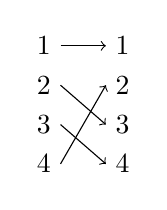
\begin{tikzpicture}
  \node (1l) at ({-1/2},2) {1};
  \node (2l) at ({-1/2},{3/2}) {2};
  \node (3l) at ({-1/2},1) {3};
  \node (4l) at ({-1/2},{1/2}) {4};
  \node (1r) at ({1/2},2) {1};
  \node (2r) at ({1/2},{3/2}) {2};
  \node (3r) at ({1/2},1) {3};
  \node (4r) at ({1/2},{1/2}) {4};
  \draw[->] (1l.east) to (1r.west);
  \draw[->] (2l.east) to (3r.west);
  \draw[->] (3l.east) to (4r.west);
  \draw[->] (4l.east) to (2r.west);
\end{tikzpicture}
\(\rho(\pi)\)\\[0pt]
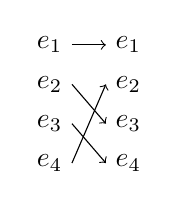
\begin{tikzpicture}
  \node (1l) at ({-1/2},2) {$e_{1}$};
  \node (2l) at ({-1/2},{3/2}) {$e_{2}$};
  \node (3l) at ({-1/2},1) {$e_{3}$};
  \node (4l) at ({-1/2},{1/2}) {$e_{4}$};
  \node (1r) at ({1/2},2) {$e_{1}$};
  \node (2r) at ({1/2},{3/2}) {$e_{2}$};
  \node (3r) at ({1/2},1) {$e_{3}$};
  \node (4r) at ({1/2},{1/2}) {$e_{4}$};
  \draw[->] (1l.east) to (1r.west);
  \draw[->] (2l.east) to (3r.west);
  \draw[->] (3l.east) to (4r.west);
  \draw[->] (4l.east) to (2r.west);
\end{tikzpicture}
Therefore\\[0pt]
\begin{align*}
  \rho(\pi)=
  \begin{bmatrix}
    1 & 0 & 0 & 0 \\
    0 & 0 & 0 & 1 \\
    0 & 1 & 0 & 0 \\
    0 & 0 & 1 & 0 \\
  \end{bmatrix}
\end{align*}
\begin{itemize}
\item Is this a group homomorphism?
\label{sec:org0eb54f8}
Let \(\pi_{1},\pi_{2}\in G\) be arbitrary elements.\\[0pt]
Need to show: \(\rho(\pi_{1}\circ\pi_{2})=\rho(\pi_{1})\circ\rho(\pi_{2})\).\\[0pt]
Both sides are linear transformations and, hence, determined by their actions on \(e_{i}\) for \(i=1,\;\ldots\;,n\).\\[0pt]
\begin{align*}
  \rho(\pi_{1}\circ\pi_{2})e_{i}
  &= e_{\pi(i)}
  \\&= e_{\pi_{1}(\pi_{2}(i))}
  \\ \rho(\pi_{1})(\rho(\pi_{2})e_{i})
  &=\rho(\pi_{1})(e_{\pi_{2}(i)})
\end{align*}
\end{itemize}
\end{itemize}
\subsection*{Composition of Group Homomorphisms}
\label{sec:orgcb55a91}
Let \(G\), \(H\) and \(K\) be groups and \(G\overset{\phi}{\to}H\) and \(H\overset{\psi}{\to}K\) be homomorphisms.\\[0pt]
Then the composite \(\psi\circ\phi:G\to K\) is a group homomorphism.\\[0pt]
\subsubsection*{Proof}
\label{sec:orgc1523af}
Let \(g_{1},g_{2}\in G\) be arbitrary.\\[0pt]
\begin{align*}
  (\psi\circ\phi)(g_{1}g_{2})
  &=\psi(\phi(g_{1}g_{2})) && \text{by definition of }\circ
  \\&=\psi(\phi(g_{1}\phi(g_{2}) && \text{since $\phi$ is a group homomorphism}
  \\&=\psi(\phi(g_{1}))\psi(\phi(g_{2})) && \text{since $\psi$ is a group homomorphism}
  \\&=(\psi\circ\phi)(g_{1})\circ(\psi\circ\phi)(g_{2}) && \text{by definition of }\circ
\end{align*}
\subsection*{Sign Homomorphism}
\label{sec:orgb2cd4ec}
Let \(n\geq1\) and \(G=\text{Sym}(n)\).\\[0pt]
Ths sign homomorphism is the composition \(\text{sign: }G\overset{\rho}{\to}\text{GL}_{n}(\R)\overset{\det}{\to}\R^{*}\)\\[0pt]
\subsubsection*{Sign of Symmetric Group}
\label{sec:org0545f7f}
\(\text{sign}(\text{sym}(n))\subseteq\{1,-1\}\leq\R^{*}\)\\[0pt]
\begin{itemize}
\item Lemma
\label{sec:orgb0b9dcc}
Let \(a_{1},\;\ldots\;,a_{m}\) be distinct numbers between \(1\) and \(n\).\\[0pt]
Then \((a_{1}\;\cdots\;a_{m})\) is equal to \((a_{1}\;\cdots\;a_{m-1})(a_{m-1}\;a_{m})\).\\[0pt]
This will be proven on homework.\\[0pt]
\item Corollary
\label{sec:orgd738a87}
Any \(m\) cycle is the composition of \(m-1\) transpositions.\\[0pt]
Namely, \((a_{1},\;\ldots\;,a_{m})=(a_{1}\;a_{2})(a_{2}\;a_{3})\cdots(a_{m-1}\;a_{m})\).\\[0pt]
Easily check: \(\text{sign}((a_{i}\;a_{i+1}))=-1\).\\[0pt]
Now any \(g\in\text{Sym}(n)\) allows a cycle decomposition.\\[0pt]
\end{itemize}
\subsection*{Kernel of a Homomorphism}
\label{sec:orge5f583d}
Let \(G\overset{\phi}{\to}H\) be a group homomorphism.\\[0pt]
The kernel of \(\phi\) is \(\ker(\phi):=\{g\in G|\phi(g)=1_{H}\}\).\\[0pt]
\subsubsection*{The Kernel is a Subgroup}
\label{sec:orgb09b233}
Let \(g_{1},g_{2}\in\ker(\phi)\). Then\\[0pt]
\begin{align*}
  \phi(g_{1}g_{2})
  &=\phi(g_{1})\phi(g_{2}) && \phi\text{ is a homomorphism}
  \\&=1_{H}1_{H} && g_{1},g_{2}\in\ker(\phi)
  \\&=1_{H} && g_{1},g_{2}\in\ker(\phi)
\end{align*}
Similarly, \(1_{G}\in\ker(\phi)\) and \(g^{-1}\in\ker(\phi)\) if \(g\in\ker(\phi)\). \(\blacksquare\) \\[0pt]
\subsection*{Alternating Group}
\label{sec:org9ba38bb}
Let \(X\) be a set, \(|X|=n\leq\infty\).\\[0pt]
The alternating group on \(X\) is the \(\text{Alt}(X)=\ker(\text{sign}:\text{Sym}(X)\to\{\pm1\})\).\\[0pt]
\section*{October 5, 2023}
\label{sec:orgdde86d0}
\subsection*{Group Action}
\label{sec:org23818e3}
Let \(G\) be a group and \(X\) a set.\\[0pt]
A (left) action of \(G\) on \(X\) is a function \(\alpha:G\times X\to X\) which satisfies two conditions:\\[0pt]
\begin{enumerate}
\item \(\alpha(1_{G},x)=x\) for all \(x\in X\).\\[0pt]
\item \(\alpha(g_{1},\alpha(g_{2},x))=\alpha(g_{1}g_{2},x)\) for all \(g_{1},g_{2}\in G\) and \(x\in X\).\\[0pt]
\end{enumerate}
\subsubsection*{Notation}
\label{sec:org6a910ab}
Write \(\alpha(g,x)=g*x=g\cdot x=gx\).\\[0pt]
\subsubsection*{Example A}
\label{sec:orgfd5b44e}
Let \(X\) be any set, and let \(G=\text{Sym}(X) = \{f:X\to X\text{ bijections}\}\) where the group operation \(\circ\) is the composition of functions.\\[0pt]
Then \(G\) acts (on the left) on \(X\) by \(f*x\underset{\text{def}}{=}f(x)\).\\[0pt]
Then the features\\[0pt]
\begin{enumerate}
\item \(\text{Id}_{X}(x)=x,\;\forall x\in X\)\\[0pt]
\item \(g_{1}*(g_{2}*x)=(g_{1}\circ g_{2})*x,\;\forall g_{1},g_{2}\in G,\;\forall x\in X\)\\[0pt]
\begin{itemize}
\item Or \(g_{1}(g_{2}(x))=(g_{1}\circ g_{2})(x)\)\\[0pt]
\end{itemize}
\end{enumerate}
are satisfied.\\[0pt]
\subsubsection*{Example B}
\label{sec:orga751d80}
Let \(G=\text{Sym}(\{B,\;P,\;W,\;Y\})\) which acts on \(X=\{B,\;P,\;W,\;Y\}\).\\[0pt]
If \(H\leq G\), then \(H\) acts on \(X\) as well, define \(h*x=\dot{h}*x\) (where \(\dot{h}\) is regarded as in the alternating group of \(G\)).\\[0pt]
In particular, \(\text{Alt}(\{B,\;P,\;W,\;Y\})\) acts on \(X\) by rotations.\\[0pt]
\subsubsection*{Example C*}
\label{sec:org9dd5610}
This example is not required for this class.\\[0pt]
From complex Analysis we have the Riemann sphere \(\mathbb{P}^{1}(\C)=\C\cup\{\infty\}\).\\[0pt]
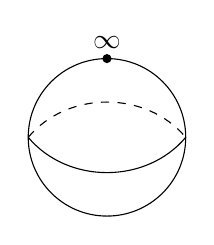
\begin{tikzpicture}
  \draw (0,0) circle (1);
  \draw[fill] (0,1) circle (0.05) node[anchor=south] {$\infty$};
  \draw[dashed] (-1,0) to[bend left=50] (1,0);
  \draw (-1,0) to[bend right=50] (1,0);
\end{tikzpicture}
Let \(G=\text{SL}_{2}(\C)\).\\[0pt]
Define \(G\)-action on \(X=\mathbb{P}^{1}(\C)\) by\\[0pt]
\begin{align*}
  \begin{pmatrix}
    \alpha & \beta \\
    \gamma & \delta
  \end{pmatrix}
  z := \frac{\alpha z+\beta}{\gamma z+\delta}
  \qquad (\infty\text{ if } \gamma z+\delta = 0)
\end{align*}
This is called the Möbius group action on \(\mathbb{P}^{1}(\C)\).\\[0pt]
Exercise: show that 1. and 2. are satisfied.\\[0pt]
\subsection*{Definitions}
\label{sec:orgda86b18}
Let \(G\) act on \(X\). (Say \(X\) is a (left) \(G\)-set)\\[0pt]
\subsubsection*{Stabilizer}
\label{sec:org815aa1f}
Let \(x\in X\). The stabilizer of \(x\) in \(G\) is \(\text{Stab}_{G}(x)=\{g\in G|g*x=x\}\subseteq G\).\\[0pt]
\begin{itemize}
\item Example 1
\label{sec:org64bb090}
Let \(G\) be any group and \(X\) a \(G\)-set.\\[0pt]
Then for any \(x\in X\), \(\text{Stab}_{G}(x)\leq G\).\\[0pt]
\begin{itemize}
\item Proof
\label{sec:org2068c26}
\begin{enumerate}
\item \(1_{G}\in\text{Stab}_{G}(x)\) since, by definition, \(1_{G}*x=x\).\\[0pt]
Therefore the identity is present.\\[0pt]
\item If \(g_{1},g_{2}\in\text{Stab}_{G}(x)\) are such that \(g_{1}*x=x\) and \(g_{2}*x=x\), then \((g_{1}g_{2})*x\underset{\text{2nd Axiom}}{=}g_{1}*(g_{2}*x)=g_{1}*x=x\).\\[0pt]
Therefore the stabilizer is closed under composition.\\[0pt]
\item Say \(g\in\text{Stab}_{G}(x)\) and \(g*x=x\). Apply \(g^{-1}\) to both sdies to get\\[0pt]
\end{enumerate}
\begin{align*}
  x\underset{\text{1st Axiom}}{=}1_{G}*x=(g^{-1}g)*x\underset{\text{2nd Axiom}}{=}g^{-1}*(g*x)=g^{-1}*x
\end{align*}
Therefore the stabilizer is closed under inverse.\\[0pt]
\end{itemize}
\item Example 2
\label{sec:org9caa7fb}
Let \(G=\text{Alt}(\{B,\;P,\;W,\;Y\})\) and consider \(H=\text{Stab}_{G}(W)=\{\text{Id},(B\;P\;Y),(B\;Y\;P)\).\\[0pt]
Fact: \(H\) does not act transitively on \(X\), since \(W\) is fixed and no element \(g\in H\) satisfies \(g*W=B\).\\[0pt]
\end{itemize}
\subsubsection*{Orbit}
\label{sec:orge17aca4}
Let \(x\in X\). The \(G\)-orbit of \(x\) in \(X\) is \(G\cdot x=\{g*x|g\in G\}\subseteq X\).\\[0pt]
Let \(G\) act on \(X\) and \(x,y\in X\). Either \(G\cdot x= G\cdot Y\) or \(G\cdot x\cap G\cdot y=\0\).\\[0pt]
So \(X\) is the disjoint union of \(G\)-orbits.\\[0pt]
e.g. \(\{B,\;P,\;W,\;Y\}=\{W\}\coprod\{B,\;P,\;Y\}\) gives the \(\text{Stab}_{G}(W)\)-orbits.\\[0pt]
\begin{itemize}
\item Example 1
\label{sec:orge1aa291}
When \(G=\text{Alt}(X)\), for \(X=\{B,\;P,\;W,\;Y\}\), there is only one orbit since \(\forall x\in X\), \(G\cdot x=X\).\\[0pt]
\item Example 2
\label{sec:org534038d}
When \(G=\text{Stab}_{G}(W)\), for \(X=\{B,\;P,\;W,\;Y\}\), then \(G\cdot W=\{W\}\) while\\[0pt]
\begin{align*}
  G\cdot B
  &=\{\text{Id}(B),\;(B\;P\;Y)(B),\;(B\;Y\;P)(B)\}=\{B,\;P,\;Y\}
  \\&=G\cdot P=\{\text{Id}(P),\;(B\;P\;Y)(P),\;(B\;Y\;P)(P)\}=\{P,\;Y,\;B\}
  \\&=G\cdot Y
\end{align*}
\end{itemize}
\subsubsection*{Transitivity}
\label{sec:org8bd2069}
Say \(G\) acts transitively on \(X\) (or the action is transitive) if, for any pair \(x,y\in X\), there exists \(g\in G\) (depending on \(x\) and \(y\)) such that \(g*x=y\).\\[0pt]
\begin{itemize}
\item Example
\label{sec:org8fe28e0}
\(G=\text{Alt}(\{B,\;P,\;W,\;Y\}) \cwcirclearrowdown \{B,\;P,\;W,\;Y\}\) is transitive.\\[0pt]
\begin{itemize}
\item Proof
\label{sec:org2eecfcb}
Let \(x,y\in X\) be arbitrary.\\[0pt]
If \(x=y\), then take \(g=\text{Id}_{X}\) and we have \(g*x=y\).\\[0pt]
Suppose \(x\neq y\), then write \(X=\{x,\;y,\;z,\;w\}\) and take \(g=(x\;y)(z\;w)\). We have \(g*x=y\).\\[0pt]
e.g. \(x=P\), \(y=Y\), \(z=B\) and \(w=W\) gives \(g=(P\;Y)(B\;W)\).\\[0pt]
\end{itemize}
\item Exercise *
\label{sec:org4724dda}
This exercise is not required for the course.\\[0pt]
Prove that \(\text{SL}_{2}(\C)\) acts transitively on \(\mathbb{P}^{1}(\C)\).\\[0pt]
Say \(\mathbb{P}^{1}(\C)\) is a homogeneous space under \(\text{SL}_{2}(\C)\).\\[0pt]
\end{itemize}
\subsection*{Group Action Gives Group Homomorphisms}
\label{sec:org231f691}
\((\longrightarrow)\) Let \(G\) act on \(X\). Then\\[0pt]
\begin{enumerate}
\item For any \(g\in G\), the function \(\pi_{g}:X\to X\) defined by \(\pi_{g}(x)=g*x\) is a bijection of \(X\), hence \(\pi_{G}\in\text{Sym}(X)\).\\[0pt]
\item The function \(G\overset{\phi}{\to}\text{Sym}(X)\) given by \(\phi(g)=\pi_{g}\) is a group homomorphism.\\[0pt]
\end{enumerate}
\subsubsection*{Proof of 1}
\label{sec:org3c5d87f}
Need to show that \(\pi_{g}\) is injective and surjective.\\[0pt]
(Inj) Let \(x,y\in X\) and assume \(\pi_{g}(x)=\pi_{g}(y)\) (i.e. \(g*x=g*y\)).\\[0pt]
Apply \(g^{-1}*\) on both sides, such that \(x=g^{-1}*(g*x)=g^{-1}*(g*y)=y\).\\[0pt]
(Sur) Let \(x\in X\) be arbitrary. Need to find \(y\in X\) such that \(\pi_{g}(y)=x\).\\[0pt]
Take \(y=g^{-1}*x\), and \(\pi_{g}(y)=g*(g^{-1}*x)=x\).\\[0pt]
\subsubsection*{Proof of 2}
\label{sec:org8ee093d}
Need to show that \(\forall g_{1},g_{2}\in G\), \(\phi(g_{1}g_{2})=\phi(g_{1})\phi(g_{2})\).\\[0pt]
\(\phi(g_{1}g_{2})\in\text{Sym}(X)\) is characterized by \([\phi(g_{1}g_{2})](x)=\pi_{g_{1}g_{2}}(x)=(g_{1}g_{2})*x\).\\[0pt]
On the other hand, \(\phi(g_{1})\phi(g_{2})\in\text{Sym}(X)\) is characterized by \([\phi(g_{1})\phi(g_{2})](x)=\phi(g_{1})[\phi(g_{2})(x)]=g_{1}*(g_{2}*x)\).\\[0pt]
By the second group action axiom, these must be the same.\\[0pt]
\subsection*{Group Homomorphism Admits Group Action}
\label{sec:org1677ef0}
\((\longleftarrow)\) Let \(G\overset{\rho}{\to}\text{Sym}(X)\) be a group homomorphism.\\[0pt]
Then, by letting \(g*x=\rho(g)(x)\in X\) we get a left \(G\)-action on \(X\).\\[0pt]
\subsubsection*{Proof}
\label{sec:org1ba6a32}
\begin{enumerate}
\item \(1_{G}*x=\rho(1_{G})(x)=\text{Id}_{X}(x)=x\).\\[0pt]
\item Let \(g_{1},g_{2}\in G\) and \(x\in X\). Then \((g_{1}g_{2})*x=[\rho(g_{1}g_{2})](x)=[\rho(g_{1})\circ\rho(g_{2})](x)=\rho(g_{1})[\rho(g_{2})(x)]=g_{1}*(g_{2}*x)\).\\[0pt]
\end{enumerate}
\subsection*{Right Group Actions}
\label{sec:orgaae87df}
Let \(G\) be a group and \(X\) be a set. A right \(G\)-action on \(X\) is a function \(\beta:X\times G\to X\) such that\\[0pt]
\begin{enumerate}
\item \(\beta(x,1_{G})=x,\;\forall x\in X\).\\[0pt]
\item \(\beta(x,g_{1}g_{2})=\beta(\beta(x,g_{1}),g_{2}),\;\forall g_{1},g_{2}\in G,\;\forall x\in X\).\\[0pt]
\end{enumerate}
\subsubsection*{Notation}
\label{sec:orga8f63dd}
\(\beta(x,g)=x*g=x\cdot g=xg\)\\[0pt]
\subsubsection*{Remark}
\label{sec:org6e0967c}
If \(\alpha:G\times X\to X\) is a left action, we get a right action \(\beta:X\times G\to X\) by \(\beta(x,g)=\alpha(g^{-1},x)\) and vice versa.\\[0pt]
That is \(x*g=g^{-1}*x\).\\[0pt]
Proof recommended as an exercise.\\[0pt]
\subsubsection*{Analogues}
\label{sec:orga669bca}
Stability, orbit and transitivty all have analogues which can be demonstrated by converting to left actions.\\[0pt]
\subsection*{Cosets}
\label{sec:orgb55c7e0}
Let \(H\leq G\), and let \(X=G\).\\[0pt]
We have left action \(H\times X\to X\) and \(h*x=hx\) (taken in \(G\)).\\[0pt]
As well as right action \(X\times H\to X\) where \(x*h=xh\).\\[0pt]
A (left) \(H\)-coset is an orbit \(xH\) for some \(x\in X\).\\[0pt]
A (right) \(H\)-coset is an orbit \(Hx\) for some \(x\in X\).\\[0pt]
\subsubsection*{Example}
\label{sec:org1170298}
Let \(G=\text{Alt}(4)\), \(H=\text{Stab}_{G}(W)=\{\text{Id},\;(B\;P\;Y),\;(B\;Y\;P)\}\).\\[0pt]
\begin{enumerate}
\item Take any \(x\in H\), \(xH=H\).\\[0pt]
\item Take \(x=(B\;P)(W\;Y)\), and \(xH=\{(B\;P)(W\;Y),(B\;P)(W\;Y)(B\;P\;Y)=(P\;W\;Y),\;(B\;P)(W\;Y)(B\;Y\;P)=(B\;W\;Y)\}\).\\[0pt]
\item There are two more; what are they?\\[0pt]
\end{enumerate}
\end{document}